\documentclass{article}


\usepackage{arxiv}

\usepackage[utf8]{inputenc} % allow utf-8 input
\usepackage[T1]{fontenc}    % use 8-bit T1 fonts
\usepackage{hyperref}       % hyperlinks
\usepackage{url}            % simple URL typesetting
\usepackage{booktabs}       % professional-quality tables
\usepackage{amsfonts}       % blackboard math symbols
\usepackage{nicefrac}       % compact symbols for 1/2, etc.
\usepackage{microtype}      % microtypography
\usepackage{lipsum}
\usepackage{float}
\usepackage{graphicx}
\usepackage{caption}
\usepackage{subcaption}
\usepackage{amsmath}
\usepackage{datetime}
\newdate{date}{13}{10}{2019}
\date{\displaydate{date}}

\usepackage{listings}
\usepackage{xcolor}	
\lstset { language=[ANSI]C++,
                backgroundcolor=\color{black!5}, % set backgroundcolor
                basicstyle=\ttfamily,
                keywordstyle=\color{blue}\ttfamily,
                stringstyle=\color{red}\ttfamily,
                commentstyle=\color{green}\ttfamily,
                morecomment=[l][\color{magenta}]{\#}
}

\title{Calvary Church Meeting \\
\large Treasury: A Summary}

\author{
  Kristoffer Lindvall\thanks{Phone: 076-761 39 20} \\
  Birgir Jarlsgatan 66B, \\
  \texttt{kristoffer.lindvall@gmail.com} \\
}
\begin{document}

\maketitle



\section{(2018) Jan - Dec}

\begin{figure}[H]
  \centering
  \begin{subfigure}{.48\textwidth}
		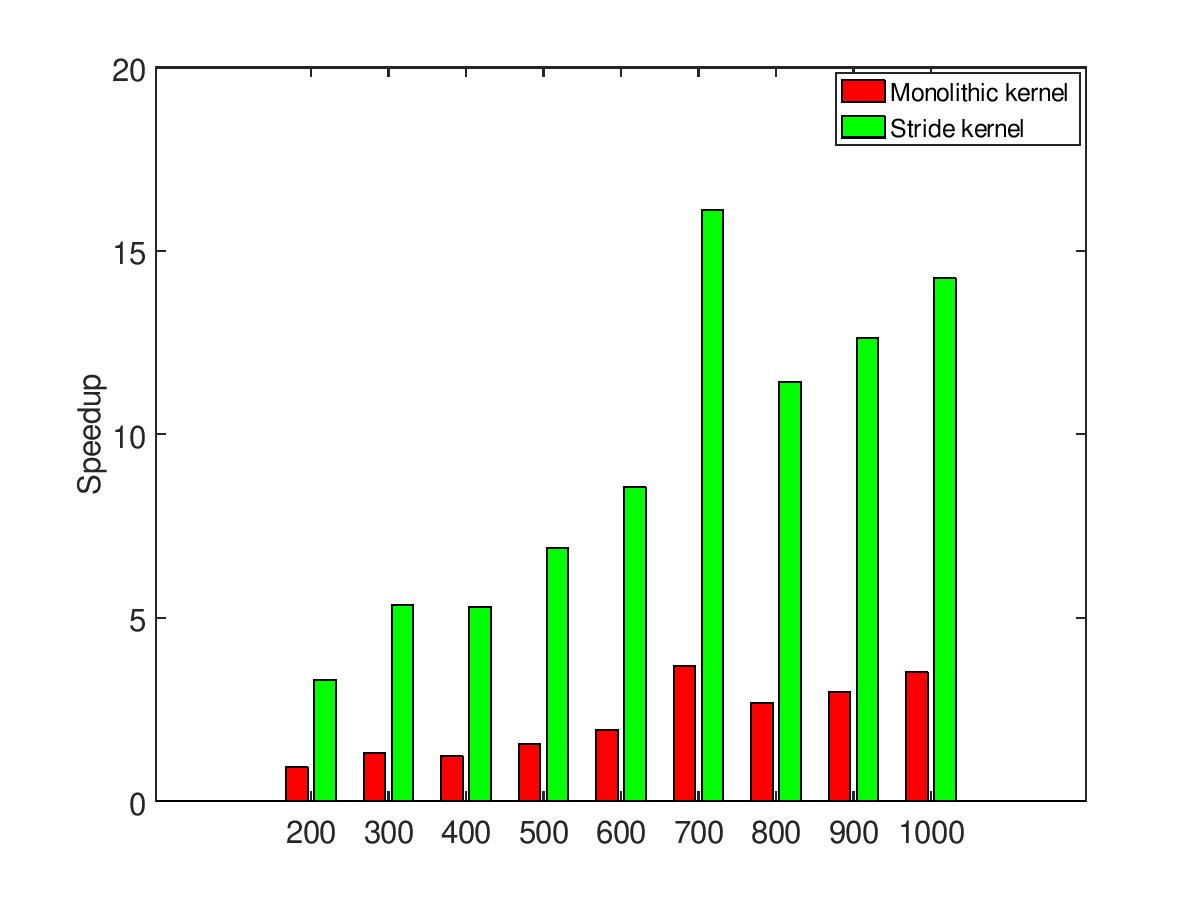
\includegraphics[width=\textwidth]{1Dparx.jpg}
		\caption{N Chebyshev modes.}
	\end{subfigure}
%%%%%%%%%%%%%%
	\begin{subfigure}{.48\textwidth}
		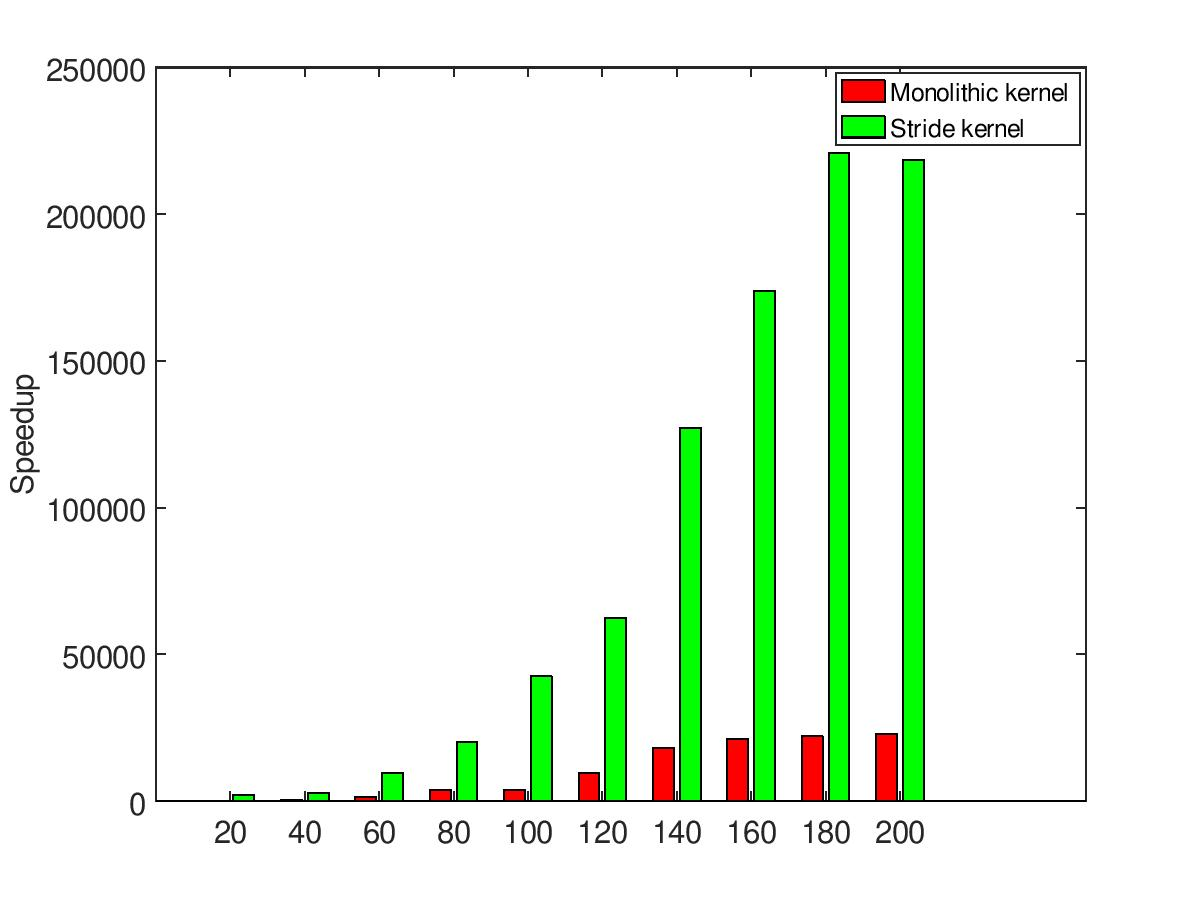
\includegraphics[width=\textwidth]{2Dpar.jpg}
		\caption{N=M Chebyshev modes.}
	\end{subfigure}
  \caption{GPU acceleration (Parallel CPU) of a 1D (a) and 2D (b) Chebyshev series product algorithm (Tesla K80). The two bars represent a naive monolithic kernel (\textit{red}) and an optimized striding kernel (\textit{green}).}
  \label{fig:fig1}
\end{figure}

\section{(2019) Jan - Oct}

\end{document}
